\section{Related Work}\label{sec:related_work}
Much work has been done to create strong models for \ac{NLI} and we show some successful strategies in Section §\ref{sec:models_snli}. Relevant datasets for \ac{NLI} are introduced in Section §\ref{sec:basics_datasets}. Before the excessive usage of neural networks, many models heavily relied on external resources, that have either been manually created in order to improve tools for \ac{NLP}, or developed in a crowd sourced manner for a different purpose, but can also be exploited. In Section §\ref{sec:ext_resources} we show an overview of some external resources that might improve the performance of neural models on \ac{NLI}. While most neural models rely solely on distributed word-representations as external information and perform quite good, prior work \citep{bos2005recognising,tatu2005semantic} depended to large degree on those resources. In Section §\ref{sec:ext_res_in_nn} we show several approaches trying to combine the power of well structured, knowledge-rich resources with the generalization power, coming from neural models with distributed word embeddings.
\subsection{External Resources}\label{sec:ext_resources}
A large variety of knowledge bases exist, containing for instance lexical relations or commonly known world knowledge, which can be helpful for improving the performance on \ac{NLI}. Research has shown that both, manually created and crowd-sourced resources, can successfully be applied in many tasks of \ac{NLP}. In this section we only show WordNet and Wikipedia, containing different information, that we consider to be useful for \ac{NLI} and \ac{NLU}, as well as two resources combining multiple resources and thus providing a huge amount of readily-available knowledge.

\subsubsection{WordNet}\label{sec:wordnet}
\begin{wrapfigure}[13]{R}{0.5\textwidth}
\centering
	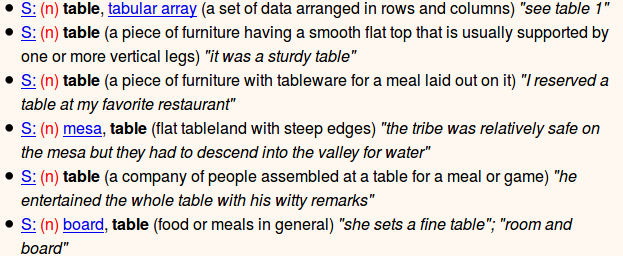
\includegraphics[totalheight=3.5cm]{fig/wordnet_example.png}
	\caption{Example of different synsets of the lemma ``table'' (only noun senses) within WordNet, taken from \href{http://wordnetweb.princeton.edu}{http://wordnetweb.princeton.edu}.}
	\label{fig:wordnet}
\end{wrapfigure}
WordNet \citep{miller1995wordnet} is a famous, manually created lexical resource for the English language, consisting of three lexica for four different \ac{POS}, one for verbs, one for nouns and one for adjectives and adverbs respectively \citep{Jurafsky2008May}. 
\paragraph*{Structure of WordNet} 
Mainly focusing on nouns\footnote{WordNet 3.0 contains 117,798 nouns, 11,529 verbs, 22,479 adjectives and 4,481 adverbs \citep{Jurafsky2008May}.} it differentiates between the more frequent class of \textit{common nouns} like ``table'' and \textit{instances} like ``Berlin''. All words are represented by their lemma and due to polysemy contain one or more senses, namely \textit{synsets}. Synsets are the main building blocks within the WordNet ontology, containing a sense description and examples. Figure \ref{fig:wordnet} displays 6 different senses for the lemma ``table''. It is noteworthy that the sense of table (as tabular array) greatly differs from the sense as ``furniture'' or ``tablelands'' while metaphorical senses strongly correlate with the sense of table as a furniture. Yet, they encode much more fine-grained sense-differences, differing only slightly from each other, compared with the difference in meaning of the first synsets. While lemmata within the same synset refer to the synonyms, other lexical semantic relations like hypernomy, antonomy and holonomy (as described in Section \ref{sec:word_relations}, however more fine-grained\footnote{For example,  WordNet differentiates between \textit{hypernyms} for common nouns and \textit{instance-hypernyms} for instances, or distinguished between \textit{part- }, \textit{member-} and \textit{substance-holonyms}.} within WordNet) are defined via labelled links between synsets. Thus, WordNet holds valuable knowledge for detecting lexical inferences in natural language.

\paragraph*{Usage and Issues}
When using WordNet in applications, one has to identify the correct sense out of many possible synsets for a given lemma. This may be done using proper algorithms for \ac{WSD}. Another simple and frequently used heuristic is to always choose the first snyset, which typically reflects the most common sense \citep{mccarthy2004using}. As shown in Figure \ref{fig:wordnet}, word-senses are defined with different granularities, that are not required by most applications. Subsequently, this reduces the interpretability of path lengths of lexical relations between two synsets. For instance, identifying that ``sunflower'' is a hyponym of ``plant'' requires the traversal over five edges (\textit{sunflower $\rightarrow$ flower $\rightarrow$ angiosperm $\rightarrow$ spermatophyte $\rightarrow$ vascular plant $\rightarrow$ plant}). At the same time, identifying that a ``church'' is a ``building'' can be identified by only traversing over two edges (\textit{church $\rightarrow$ place of worship $\rightarrow$ building}) and traversing similarily over five edges leads to the synset ``whole, unit'', covering both, living things and objects. This is a known issue \citep{resnik1995using} and strategies have been proposed to reduce the complexity of WordNet, if the specific domain is known, for instance using sense clustering \citep{prakash2007learning}.

\subsubsection{Wikipedia}\label{sec:wikipedia}
While WordNet contains manually annotated lexical relations and is easily and automatically accessible, Wikipedia\footnote{\href{https://www.wikipedia.org/}{https://www.wikipedia.org/}} is a huge multi-lingual, continuously growing  encyclopedia, maintained by many volunteers. Also mostly focusing on nouns, due to the nature of containing encyclopedic information, it contains a large variety of factual information about named entities, that many other lexical resources lack \citep{gurevych2016linked}. Even though it has not been created for the purpose of serving as a lexical knowledge base, it still may be seen as  partially annotated resource, due to artifacts like hyperlinks. These can be interpreted similarily and even accessed using available tools in a programmatic manner \citep{zesch2008extracting}.  \cite{gurevych2016linked} describe the following information types that can be exploited to retrieve lexical information:
\begin{itemize}
\item \textbf{First paragraph:} The first paragraph of an article can be interpreted as the \textit{sense definition}, since every article covers only one aspect due to the nature of encyclopedias.
\item \textbf{Hyperlinks:} \textit{Sense examples} can be retrieved from the context, surrounding a hyperlink that links to the entity of interest, showing how the term is used.
\item \textbf{Hyperlinks:} Hyperlinks between articles can be considered as \textit{sense relations}.
\item \textbf{Translation Pages:} Due to interlinked articles in different languages, the corresponding titles usually can serve as \textit{translation equivalents}.
\end{itemize}
Wikipedia has successfully been used in many applications for \ac{NLP} and even though we do not conduct experiments within this work using Wikipedia, it clearly contains rich factual and world knowledge, that can be helpful for \ac{NLI} systems. 
\subsubsection{Derived from multiple Knowledge Bases}
\ac{YAGO} \citep{suchanek2007yago} combines the high coverage of Wikipedia with the clean taxonomy of WordNet, leading to a very knowledge rich resource. \ac{YAGO} mainly targets to contain a large amount of world-knowledge with Wikipedia, as being tremendously larger than WordNet, and additionally contains relations to express facts derived from it. As opposed to \ac{YAGO}, UBY \citep{gurevych2012uby} aims for lexical semantic richness. In addition to Wikipedia and WordNet, seven other resources are combined together, providing lexical semantic knowledge in German and English. The combination is realized by using so-called \textit{sense axis}, links between two senses of different lexicons. UBY provides an easy-to-use API, making its high-coverage knowledge programatically accessable to \ac{NLP} applications. Having these knowledge-rich resources available, but for the most part decoupled from neural approaches, still lacking this exact knowledge, stresses the benefit of combining these two worlds. 

\subsection{Datasets for NLI}\label{sec:basics_datasets}
As neural models usually require a huge amount of data for their training, they were not successfully applicable to \ac{NLI} tasks until the release of \ac{SNLI}, reaching state-of-the-art results. Previous \ac{NLI} tasks like FraCas \citep{cooper1996using} or the PASCAL challenge \citep{dagan2006pascal} only consisted of a very limited amount of training data. Some datasets, like \ac{SICK} \citep{marelli2014semeval} or the Denotation Graph entailment set \citep{young2014image}, increased the amount of samples at the expense of using artificially created sentences and/or automatically labeling, reducing the textual quality and adding noise. Since the focus in this work is on neural models, only the relevant datasets for this purpose are introduced.
\subsubsection{SNLI}\label{sec:snli}
With the release of \ac{SNLI} \citep{bowman2015large} researchers were able to apply neural models for the task of \ac{NLI} using distributed word-representations. The corpus consists of 570,152 human written sentence pairs and differentiates between the three labels, described in Section §\ref{sec:basics_nli}. 
\paragraph*{Event co-reference}
A drawback of all previsously existing resources for \ac{NLI}, that is handled by \cite{bowman2015large}, is the fact that even humans may assign different labels to a sentence pair, based on their subjective interpretation, that all can be valid. This issue can be demonstrated using the following sentence pair:
\begin{center}
\begin{tabular}{rl}
\textbf{Premise:} & Young people are demonstrating in San Francisco.
\\
\textbf{Hypothesis:} & Young people are demonstrating in New York.
\end{tabular}
\end{center}
One could clearly argue the sentence-pair should be labelled as \textit{neutral}, since there could be people demonstrating in both cities. However, it is also legimate to interpret these as contradicting sentences, if one considers both sentences to be describing the same event. While both sentences may be true when describing different potential scenarios, only one of them can be true, if they refer to the same. In order to reduce noise coming from these inconsistent interpretations, the labeling scheme within \ac{SNLI} must be fixed beforehand. Specifically they choose the labelling scheme to be based on event-coreference, the latter of the two explanations, as otherwise only very general statements would result in \textit{contradiction}.
\paragraph*{Generation}
In order to create \ac{SNLI}, \cite{bowman2015large} used image captions from the Flickr30k corpus \citep{young2014image} as premises and let human workers create hypothesis for each label respectively, using Amazon Mechanical Turk, by asking them to write alternative captions that
\begin{itemize}
\item definetely also are a true description of the photo  \textbf{(entailment)}
\item might be a true description of the photo \textbf{(neutral)}
\item definetely are a false description of the photo \textbf{(contradiction)}
\end{itemize}
The workers only saw the image caption, not the image itself, but were encouraged to use common world knowledge, enabling the creation of inferences that require additional information of the world, that is not available in word-embeddings\footnote{For instance (taken from \ac{SNLI}) \textit{snow} is paraphrased as \textit{frozen particles of water} and requires factual knowledge to be understood correctly.}. While this process simplifies the task of assuming event-coreference, the sentences within \ac{SNLI} are rather simple and short, due to the nature of image captions. 

\paragraph*{Looking into data}
As we conduct most of the experiments of this work on \ac{SNLI}, it is important to get an understanding of how sentences in this dataset look like. As previously mentioned, the vast majority of sentences are rather simple and might even be phrases only, rather than proper sentences, due to omission of a verb. In addition to that, sentences might be written in proper English, but also might contain spelling or punctuation errors, be lowercased only, or describe highly unrealistic scenarios.  Table \ref{table:snli_example} shows selected sample sentence-pairs, taken from the \ac{SNLI} dataset.
\begin{center}
\begin{table}[htt]
\begin{center}
\resizebox{\textwidth}{!}{%
\begin{tabular}{lll}
\textbf{Premise} & \textbf{Hypothesis} & \textbf{Label} \\
\toprule
\multirow{3}{*}{\textbf{(1)} The large brown dog jumps into a pond.} & The dog is getting wet. & \textit{entailment} \\ & The dog is a chocolate Labrador Retriever. & \textit{neutral} \\
&A white cat is sunning itself on a windowsill. & \textit{contradiction} \\
\midrule
\multirow{3}{*}{\textbf{(2)} A woman is handing out fruit.} & A woman is passing out different types of fruits. & \textit{entailment} \\
&A woman is handing out oranges. & \textit{neutral} \\
&A fruit is handing out a woman. & \textit{contradiction} \\
\midrule
\multirow{3}{*}{\textbf{(3)} A basketball game.} & A sports game. & \textit{entailment} \\
&A basketball game between rivals. & \textit{neutral} \\
&A volleyball game. & \textit{contradiction} \\
\bottomrule
\end{tabular}}
\end{center}
\caption{Example sentence pairs, taken from \ac{SNLI}, showing typical sentences within the dataset.}
\label{table:snli_example}
\end{table}
\end{center}
The first column displays the premise, in the second column three hypothesis are shown, created by the workers for each label respectively. Several characteristics of the dataset and types of required knowledge to solve the task can be seen here. 
The first examples \textbf{(1)} require the model to have some factual knowledge that a ``Labrador Retriever'' is some kind of ``dog'', and ``chocolate'' is paraphrasing ``brown''. Since ``Labrador Retriever'' is a possible substitute for ``dog'' but more specific, the sample is labelled as neutral. The according entailing hypothesis requires an even deeper understanding of the world, as the system needs to know, that a ``pond'' is filled with water and anything that goes into water is ``getting wet''. The contradicting sample shows two frequently occuring characteristics. Not only has ``dog'' been replaced by ``cat'', but also the color and the activity changed. We found that in many contradicting hypothesis several contradicting words with respect to the premise exist, obviously making the task easier, as it is sufficient to only detect one of these indicators. Additionally, it has been shown, that the creation process of the hypothesis followed some heuristics, shared by many workers\citep{gururangan2018annotation}. Specifically the replacement of ``dog'' to ``cat'' occurs often enough, that the presence of ``cat'' in the hypothesis alone is a strong indicator for contradiction already. 
\newline

\noindent
The sentences of the second example \textbf{(2)} are based on paraphrasing, representing the same meaning, (entailment), have more specific term in the hypothesis as in the premise (neutral), and show semantic role reversal (contradiction),  which is somewhat interesting, as it requires to model to leverage word order. A simple \ac{BoW} approach would fail here.
\newline

\noindent
In contrast to \textbf{(1)} the sentences in \textbf{(3)} only require very shallow knowledge. Here, the word ``basketball'' is substituted by its' hypernym\footnote{At least in one sense, not in the sense of \textit{being a ball}.} ``sport'', thus still covering the original meaning by being more general. The next sentence gives some plausible additional information not given in the premise, hence neutral. In the last contradicting sentence, the model has to identify that ``basketball'' and ``volleyball'' are mutually exclusive, which shows, how co-hyponyms influence the relation label. While sentences are often a bit longer than in this example, the required knowledge, as specified in \textbf{(3)}, is most present within \ac{SNLI}.

\subsubsection{MultiNLI}
\ac{SNLI} received some critizism within the research community \citep{chatzikyriakidis2017overview,williams2017broad}, mainly due to its' simplicity, coming from the fact, that all premises are taken from a single genre only, namely image captions. Thus, \ac{SNLI} is very limited to only visual scenes, neglecting many other aspects like temporal reasoning, modality or belief. \cite{williams2017broad} introduced with \ac{MultiNLI} a new dataset, overcoming these drawbacks. 
\paragraph*{Generation of \ac{MultiNLI}}
The authors followed the same generation procedure, as has been done by \cite{bowman2015large}, but instead of relying on image captions only, they took into considerations other genres from \ac{OANC}\footnote{Genres from \ac{OANC}: \textit{Government, Slate, Telephone Speech, Travel Guides, 9/11 Report, Face-to-face Speech, Letters, Nonfiction Books, Magazine}} \citep{ide2001american,ide2004american,ide2006integrating} as well as several freely available fiction work, resulting in 10 additional genres with 392,702 new sentence-pairs for training and 20,000 for development and test respectively. A major motivation for the creation of \ac{MultiNLI} was, to put more emphasis on the role of \ac{NLI} as evaluation benchmark of \ac{NLU} that \ac{SNLI} failed to provide due to its narrow coverage. Therefore, only five of the new genres are present within the train data, while the remaining five genres only occur in the test set, serving as evaluation for cross-domain transfer learning and domain adaption. The performance on this dataset is measured in two figures, \textit{matched} examples are derived from the same source as training samples, while \textit{mismatched} examples differ from those seen during the training (containing the additional genres). This motivation becomes also clear from the corresponding Shared Task \citep{nangia2017repeval}, allowing any kind of external resources (including the ones that were used to derive the premises) but only accepting sentence-encoding models\footnote{These models encode each sentence individually and are explained in Section §\ref{sec:models_snli}.} to evaluate sentence-representation learning with respect to \ac{NLU}. \ac{MultiNLI} has been shown to be harder than \ac{SNLI} \citep{williams2017broad}, the best performing model of the RepEval 2017 Shared Task reaches 74.9\% matched and mismatched accuracy \citep{chen2017recurrent} using ensembles and 74.5\% matched, 73.5\% mismatched accuracy using a single model\citep{nie2017shortcut}. 
\paragraph*{Looking into data}
Table \ref{table:multinli_example} depicts a few samples of different genres\footnote{Taken from https://repeval2017.github.io/shared/}. One can see how different genres broaden the scope of language that is used to express inferences. A system needs to deal with temporal information and less visualizable terms like \textit{appreciate} or \textit{benefit}.
\begin{center}
\begin{table}[h]
\begin{center}
\resizebox{\textwidth}{!}{%
\begin{tabular}{llll}
\textbf{Premise} & \textbf{Hypothesis} & \textbf{Label}  & \textbf{Genre} \\
\toprule
\multirow{3}{*}{\parbox{6cm}{The Old One always comforted Ca'daan, except today.}} & \multirow{3}{*}{\parbox{6cm}{Ca'daan knew the Old One very well.}} & & \\
& & \textit{neutral} & Fiction \\
& & & \\
\midrule
\multirow{3}{*}{\parbox{6cm}{Your gift is appreciated by each and every student who will benefit from your generosity.}} & \multirow{3}{*}{\parbox{6cm}{Hundreds of students will benefit from your generosity.}} & &\\
&  & \textit{neutral} & Letters \\
& & & \\
\midrule
\multirow{3}{*}{\parbox{6cm}{At the other end of Pennsylvania Avenue, people began to line up for a White House tour.}} & \multirow{3}{*}{\parbox{6cm}{People formed a line at the end of Pennsylvania Avenue.}} &  & \\
& & \textit{contradiction} & 9/11 Report \\
& & & \\

\bottomrule
\end{tabular}}
\end{center}
\caption{Example sentence pairs from \ac{MultiNLI}, taken from RepEval 2017 Shared Task, showing samples of different genres.}
\label{table:multinli_example}
\end{table}
\end{center}
As the authors followed the same guidelines as in \ac{SNLI}, and also assume event-coreference, both datasets are highly compatible, only differing in the range of genres and thus diversity of language. \ac{MultiNLI} is even distributed in the same data format and a common practice is, to include data from \ac{SNLI} when training models for \ac{MultiNLI} \citep{nie2017shortcut,balazs2017refining,yang2017character}.

\subsubsection{SciTail}
SciTail \citep{scitail} is yet another dataset for \ac{NLI}, designed to address a different problem of previously existing datasets\footnote{Ignoring small-scale datasets with less than 1,000 samples.}. The targeted problem of previous work, including \ac{SNLI} is, that either the premise or the hypothesis was specifically for this task created, thus neglecting the kind of naturally occuring inference problems of any endtask like \ac{QA}. It is comparably smaller, consisting of only 27,026 examples and only distinguishes between two labels, \textit{entailment} and \textit{neutral}. \textit{Entailment} is defined as in \ac{SNLI} and \ac{MultiNLI}, saying that the premise supports the hypothesis. All cases where the hypothesis is not supported by the premise however, are classified \textit{neutral}.

\paragraph*{Generation of SciTail}
In order to retrieve premise and hypothesis from a resource, rather than creating one sentence for the specific purpose of \ac{NLI}, \cite{scitail} took a different approach to generate the corpus. The dataset originates from school-level multiple-choice questions for science \ac{QA} \citep{welbl2017crowdsourcing}. Those questions generally require sophisitcated reasoning capabilities in order to answer them correctly. 
\begin{enumerate}
\item \textbf{Hypothesis:} Given the short factual answer-candidates and a question, a new sentence was synthesized using the question and answer. This sentence serves as the hypothesis. For instance the question ``When waves of two different frequencies interfere, \textit{what phenomenon occurs?}'' and the correct answer ``beating'' is transformed into ``When waves of two different frequencies interfere, \textit{beating occurs}'' \citep{scitail}.
\item \textbf{Premise:} A large background corpus with relevant information from \cite{clark2016combining} was used to generate candidate knowledge sentences for each question using \ac{IR} for the premise.
\item \textbf{Label:} While hypothesis, derived from an incorrect answer, can be assumed to be not-supported by the premise, those derived from a correct answer are not necessarily supported by the premise. Thus, samples where croud-sourced annotated, to ensure a correct labelling, only keekping those samples as entailment, that were labelled to have \textit{Complete Support}\footnote{Annotators could decide between \textit{Complete support} (labelled as entailment), \textit{Partial Support} (ignored) and \textit{Unrelated} (labelled as neutral).}.
\end{enumerate}
Due to its relatedness with Scientific \ac{QA}, the authors claim, that a model reaching a good performance on this dataset for \ac{NLI} will also score well on an according \ac{QA} task, as similar \ac{NLU} is needed. SciTail is different in nature to the two previous datasets. Neither does it contain contradicting examples, nor does it assume event-coreference, as sentence-pairs in this dataset are more based on factual information. 


\subsection{Neural Models for NLI}\label{sec:models_snli}
We follow the \ac{SNLI} leaderboard\footnote{https://nlp.stanford.edu/projects/snli/} by differentiating between \textit{sentence-encoding} and \textit{inter-sentence-attention} based models. In the following, we show an overview about relevant approaches of both areas. The Residual- or Shortcut-Stacked Encoder, as introduced in Section §\ref{sec:residual_encoder_def}, belongs to the former class of models. 
\subsubsection{Sentence Encoding Models}
Sentence-encoding models follow the Siamese Architecture \citep{bromley1994signature}, meaning they encode both, sentences $p$ and $h$, individually, with parameters being tied between both sentence encoders. The inference classification is predicted by a following classifier like a \ac{MLP}. Doing so, the models put more emphasis on a meaningful sentence representation with the motivation of being generally applicable and less focused on the specifc characteristics of the task at hand \citep{bowman2016fast}. Many different strategies are used to create meaningful sentence representations within this class of neural models. This is for instance done by exploiting syntactical information using neural Shift-Reduce-Parsers, that create a linear sequential structure from tree-structured sentence representations \citep{bowman2016fast}, or by adding external memory with read- and write-operations, capturing the temporal and hierarchical information within natural language \citep{munkhdalai2017neural}. 

\paragraph*{Inner-attention-based models}
Following the intuition that humans only remember certain parts of a sentence after reading it, \cite{chen2017recurrent} model this human behaviour using gated intra-sentence attention, by generating the sentence representation via pooling\footnote{As done with max-pooling by \cite{nie2017shortcut}.} strategies over the outputs of the encoding \ac{biLSTM}. The outputs are reweighted using  attention gates. The idea of using inner-attention mechanisms is also used by the best performing sentence encoders for \ac{SNLI}, at the time of this writing reaching 86.3\% in accuracy \citep{shen2018reinforced,im2017distance}. \cite{shen2018reinforced} create sentence representations using the combination of hard and soft self-attention\footnote{A plain attention function calculates the alignment for an input sequence $x=[x_1, x_2, ...,x_n]$ given a query $q$. In the special case of self-attention, $q$ arises from the input sequence $x$ itself \citep{shen2018reinforced}.}. While hard-attention forces the model to only focus on relevant elements of the input sequence, disregarding all other elements, it is not fully differentialbly and thus inefficient to train. Soft-attention methods on the other hand, are fully differentiable and weight each element of the input sequence according to their relevance. However, by also giving positive, non-zero weights to irrelevant elements, it diminishes the emphasis on truely important ones. By first applying hard-attention to retrieve a subset of context-aware elements, that is afterwards processed using soft-attention, \cite{shen2018reinforced} leverage the mentioned advantages of both techniques. Inner attention is also used by \cite{im2017distance}, however their model additionally uses directional masks, that prevent the network from considering following or preceeding words in the attention process respectively. Furthermore, they use distance masks, that reduce the attention weights, if words are further away from each other. They show that their model outperforms others, especially with longer input sentences, as the result of considering word distance and positional information.

\subsubsection{Inter-sentence-attention-based models}\label{sec:rel_work_sentence_encoding_models}
\cite{rocktaschel2015reasoning} shows, that models perform significantly better, when looking at both sentences simultaneously in the sentence-encoding step. This is motivated by the way, humans would solve the task of \ac{NLI}, by first reading the premise, and creating the understanding of the hypothesis based on the previously read sentence. Since this seems to be superior in \ac{SNLI}, many works follow this approach, reaching state-of-the-art results. Also in this class of methods memory networks, accessable via attention, were applied \citep{cheng2016long}.

\paragraph*{Inter-sentence-attention-based models used within this work}
\cite{parikh2016decomposable} provide a simple network structure, called \textit{Decomposable Attention}, using the assumption that only parts of a sentence are needed for the entailment relationship. They do so by fragmenting the input sentences into subphrases and align the fragments of both sentences with each other using attention. Even though they represent sentences in a \ac{BoW} manner, they reach a remarkable performance. After comparing the aligned phrase-pairs, the final sentence representation is retrieved by a simple summation over the comparison-vectors from the previous step. Thus, by using this rather basic aggregation method rather than relying on any \ac{LSTM}-based method, they reduce computational complexity tremendeously. \ac{ESIM} \citep{chen2017enhanced} is another simple yet strong model, essentially consisting of three different steps. First, words are encoded using \ac{biLSTM}s such that they represent the context as well as the word itself. Next, similarily to \cite{parikh2016decomposable}, they calculate the local inference between elements in both sentences, by reweighting the sentence representations, based on the normalized attention weights. They enhance this information, using the feature concatenation of \cite{mou2015natural}, as done in the Shortcut-Stacked Encoder, however in this approach word order information is preserved by the network, in contrast to Decomposable Attention. The final sentence representation is created using pooling\footnote{As opposed to summation in Decomposable Attention. \cite{chen2017enhanced} evaluate in their experiments, that pooling leads to superior results than summation, due to being less sensitive to the sentence length.} on the ouput of a \ac{biLSTM}, composing the local inference information from the previous step. The composed vector is finally fed into a \ac{MLP} classifier for the prediction. \cite{chen2017enhanced} report their results using an ensemble of two implementations with the same base architecture. One, as described here, relies on a \ac{biLSTM}, the other focuses more on syntactic features by encoding sentences with a TreeLSTM. While Decomposable Attention and ESIM achieve competitive results on \ac{SNLI} we conduct experiments using both models in Section §\ref{sec:additional_snli_set}, showing that these results are rather a matter of memorization than generalization.

\paragraph*{Attempt to incorporate WordNet}
Very recently, \cite{chen2017natural} introduced with \ac{KIM} a neural model, incorporating information from WordNet. This is, at the time of this writing,  the single best performing model on \ac{SNLI}. In their approach, they map WordNet relations, as defined in Section §\ref{sec:word_relations}, to a real number $r \in \mathbb{R}$ with $0 \leq r \leq 1$, quantifying the relations between word within $p$ and $h$ based on the path length of each relation within WordNet, and represent each word-pair with this additional feature vector. However even by enrichening the representations with WordNet information, they only outperform models without external information by a small margin, ranging from 0.1 to 0.6 points in accuracy. \cite{chen2017natural} show that adding WordNet is helpful if less train data is available, however only show limited evidence, that the model leverages from WordNet fused relations for the overall improvement in accuracy\footnote{This is true for the first published version \citep{chen2017natural}. Subsequentially to work presented within this thesis in Section §\ref{sec:additional_snli_set}, they show indeed that the additional information from WordNet is a key factor within \ac{KIM} in their updated version \citep{chen-EtAl:2017b:natural}.}. In this paper we show that performance on \ac{SNLI} is not sufficient evidence for the capability of dealing with simple lexical inferences as inferred from WordNet, which suggests that further investigations should be conducted in this direction.

\paragraph*{Benchmark}
To this date, the best single sentence-encoding models on \ac{SNLI} reach 88.6\% \citep{chen2017natural} ensembles reach up to 89.3\% \citep{tay2017compare,peters2018deep,ghaeini2018dr} giving an advantage of 2.3\% or 3.0\% respectively over the best sentence-encoding model \citep{im2017distance}. Considering that the human performance on \ac{SNLI} only is estimated to be 87.7\% \citep{gong2017natural} indicates, that research started to slightly overfit on the dataset already. 

\subsection{Integration of external Resources into Neural Networks}\label{sec:ext_res_in_nn}
There have been several approaches to integrate knowledge of different kind (as described in Section §\ref{sec:basics_datasets}) into neural networks. \cite{hu2016deep} infer external knowledge, represented in logical form, using a student-teacher setup. In this setting, the teacher, a neural network, is constrained by the rules acquired from an external resource. The student, also a neural network, considers two labels: the true labels and the constrained predictions of the teacher. By simultaneous training both networks influenced by each others predictions, the logical rules are integrated within the networks parameters, weighted by their learned relevance (soft rules rather than scrict hard rules). Most attempts to incorporate external information however, do so by enhancing word representations.
\subsubsection{Improving word-embeddings}\label{sec:embeddings_improvements_relwork}
A very intuitive way to integrate external resources is, to enrich word-embeddings with additional information. As most neural models depend on vector representations for words anyway, improvement of word-representations can be adapted with very limited effort to most models.

\paragraph*{Joint learning of distributional embeddings with external information}
\cite{xu2014rc} differentiate between \textit{categorical} (attributes of words like the ``gender'') and \textit{relational} (relations between words, like ``child-of'', ``is-a'', e.t.c.) knowledge and train the word-embeddings from scratch, using three objective functions simultaneously. They use skip-gram\footnote{Skip-gram essentially optimizes the prediction of the probability of context-words appearing in the (close) context of a target word \citep{goldberg2014word2vec}.} to encode distributional properties. At the same time, they minimize the distance between words, that share the same category, thus clustering words by their categorical similarities. Third, they represent a relation as a vector $r$,  and optimize word vectors, such that for a word $w_1$, connected to another word $w_2$ via relation $r$ the equation $w_1 + r \simeq w_2$ holds. \cite{liu2015learning} construct enriched embeddings by defining it as a constrained optimization problem. Specifically, they create constraints by ranking word similarities such that, for instance synonyms should be more similar than antonyms or hyponyms should be more similar to close hypernyms than to distant hypernyms. Finally they include those contraints into the training process with skip-gram. 
\paragraph*{Post-processing existing representations}
 \cite{faruqui2015retrofitting} propose a method called \textit{Retrofitting}, a post-processing method than can be applied on any pre-trained word-representations. They reduce the eucledian distance between words, that are connected with a lexical semantic relation within a resource, while also keeping the representations close to the original neighbouring word-representations. Attract-Repel \citep{mrkvsic2017semantic} is another retrofitting method, essentially pulling synonyms closer to each other while pushing antonyms further apart in vector space, while trying to keep the original distributional information. Similarily \cite{vulic2017specialising} build on attract-repel, adding hypernym relations for the context of lexical entailment, by using an asymmetric distance measure between hypernym-hyponym pairs.
 
\paragraph*{Effectiveness of improved representations}
The demand of integrating lexical resources such as WordNet has mainly been targeted by enrichening word-representations, with previously mentioned approaches being just a small selection. The improvement over standard distibutional word-embeddings of most of these approaches however, is either demonstrated by visualizing word-relation vectors, that may not even be expoited by end-to-end neural networks \citep{levy2015improving}, or based on evaluations on very low-level tasks like Word-Similarity, Syntactic Relations or Analogical Reasoning, or, by solely providing intrinsic evaluations. Neural networks for higher level tasks like \ac{NLI} however, reach state-of-the-art performances, still relying on standard pre-trained distributional word-representations like GloVe, even though alternatives exist. Prelimitary experiments\footnote{These experiments have been conducted by Vered Shwartz in prior work and are not part of this work.} of using enriched embeddings for \ac{SNLI} have shown no success. We evaluate the possibility of adding enriched embeddings, following the successful idea of \cite{ruckle2018concatenated}, that different embeddings encode complementary information, by concatenating different word-representations. However we focus our experiments on the integration of knowledge on a more progressed step of the network, the sentence representation, due to limited reported success on end tasks using richer embeddings, though many of those embeddings exist.
%\citep{iacobacci2015sensembed} sense embeddings + drawback polysemy
%\citep{rothe2015autoextend} autoexten +WordNet (i think)
%\citep{toutanova2015representing} jointly and \citep{zhong2015aligning}
